% !TEX encoding = UTF-8
% !TEX TS-program = pdflatex
% !TEX root = ../tesi.tex
\newpage
%**************************************************************
\chapter{Obiettivi dello stage}
\label{cap:obiettivi-stage}
%\intro{Brevissima introduzione al capitolo}\\
%%%%%%%%%%%%%%%%%%%%%%%%%%%%%%%%%%%%%%%%%%%%%%%%%%%%%%%%%%%%%%%%%%%%%%%%%%%%%%%%%%%%%%%%%%%
\section{Lo stage nella strategia aziendale}
%Importanza dello stage in AzzurroDigitale
%%%%%%%%%%%%%%%%%%%%%%%%%%%%%%%%%%%%%%%%%%%%%%%%%%%%%%%%%%%%%%%%%%%%%%%%%%%%%%%%%%%%%%%%%%%
\subsection{Vantaggi Aziendali}
%Vantaggi per l'azienda: \\
%- partecipazione a stageIT consente all'azienda di entrare in contatto con i laureandi\\
%- formazione di personale giovane e selezionato\\
%- nuove idee e punti di vista \\
%%%%%%%%%%%%%%%%%%%%%%%%%%%%%%%%%%%%%%%%%%%%%%%%%%%%%%%%%%%%%%%%%%%%%%%%%%%%%%%%%%%%%%%%%%%
\subsection{Presentazione dei progetti}
%descrizione generale dei progetti: \\
%- le idee che stanno dietro a questi\\
%- peculiarità\\
%- differenze con la concorrenza\\
%%%%%%%%%%%%%%%%%%%%%%%%%%%%%%%%%%%%%%%%%%%%%%%%%%%%%%%%%%%%%%%%%%%%%%%%%%%%%%%%%%%%%%%%%%%

\begin{figure}[h]
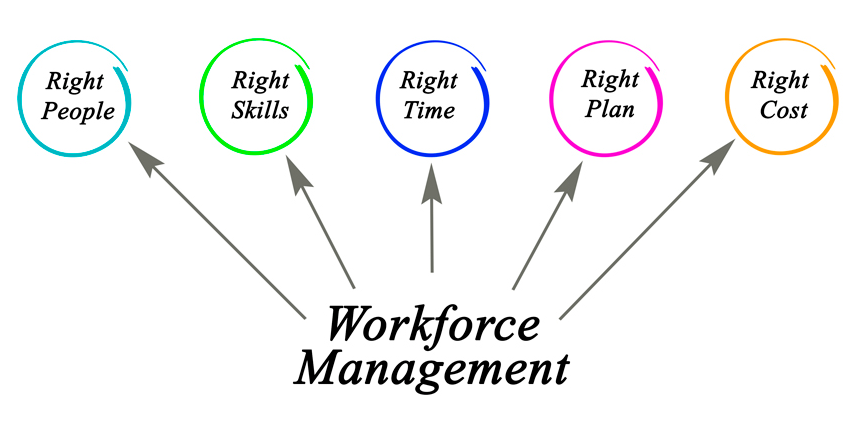
\includegraphics[width=0.9\textwidth]{workforce-management.png}
\centering
\caption{Concetti di \textit{Workforce Management}.} 
\source{\href{https://www.replgroup.com/}{Replgroup.com}}
\label{fig:workforce-management}
\end{figure}


\subsection{Aspettative aziendali}
%definizione e classificazione degli obiettivi da raggiungere

Presentati i progetti, si è passati alla fase di definizione dei traguardi da raggiungere durante lo stage.
Il team di sviluppo ha deciso di suddividere questi obiettivi in due categorie: gli \textbf{obiettivi minimi} si riferiscono a dei compiti il cui completamento risulta essere indispensabile per l'avanzamento del progetto, gli \textbf{obiettivi opzionali} invece, fanno riferimento a delle caratteristiche del prodotto di importanza minore e quindi il loro soddisfacimento non è stato considerato obbligatorio.
Di seguito, il riepilogo degli obiettivi che mi sono stati assegnati, ripartiti tra i vari progetti.

\subsubsection*{DigitalSnapshots}
\paragraph*{Obiettivi Minimi}
\begin{itemize}
\item Ristrutturazione della base di dati MySQL e della parte Model di CakePHP;
\item Realizzazione moduli API e logica;
\item Creazione interfaccia utente del cruscotto delle analisi; 
\item Stesura della documentazione su quanto realizzato.
\end{itemize}

\paragraph*{Obiettivi Opzionali}
\begin{itemize}
\item Realizzazione di un modulo \textit{wizard} per la configurazione rapida del prodotto;
\item Implementazione di una gerarchia di utenti, con livelli di privilegi differenti.
\end{itemize}

\subsubsection*{AWMS}
\paragraph*{Obiettivi Minimi}
\begin{itemize}
\item Implementazione dei dati necessari nel database PostgreSQL e nella parte Model di CakePHP;
\item Realizzazione moduli API e logica;
\item Creazione interfaccia utente per la selezione della tipologia e delle opzioni di stampa; 
\item Stesura della documentazione su quanto realizzato.
\end{itemize}

\paragraph*{Obiettivi Opzionali}
\begin{itemize}
\item Realizzazione di un modulo per la configurazione dei ruoli degli utenti;
\item Implementazione di un algoritmo per la pianificazione intelligente della forza lavoro a disposizione.
\end{itemize}

\section{Vincoli}
\subsection{Vincoli temporali}
%ore di lavoro complessive, scadenze sprint e scadenze di progetto

La durata complessiva dell'attività di stage è stata di 304 ore, distribuite, in accordo con il tutor aziendale, nell'arco di 8 settimane, ognuna delle quali aveva un monte orario di circa 40 ore. \\
L'orario lavorativo stabilito corrisponde all'orario di lavoro aziendale: dal Lunedì al Venerdi, dalle ore 9:00 alle 18:00.\\
Oltre a questo vincolo del monte orario, mi sono trovato a toccare con mano la pianificazione Scrum: all'inizio di ogni Sprint, infatti, ho pianificato le attività da portare a termine entro le successive due settimane, durata di ogni singolo Sprint.//
Il progetto \textbf{DigitalSnapshots} inoltre, aveva una scadenza di consegna al cliente che combaciava con la fine del secondo Sprint, per cui il ritmo lavorativo è stato abbastanza elevato per non eccedere tale data.

\begin{figure}[h]
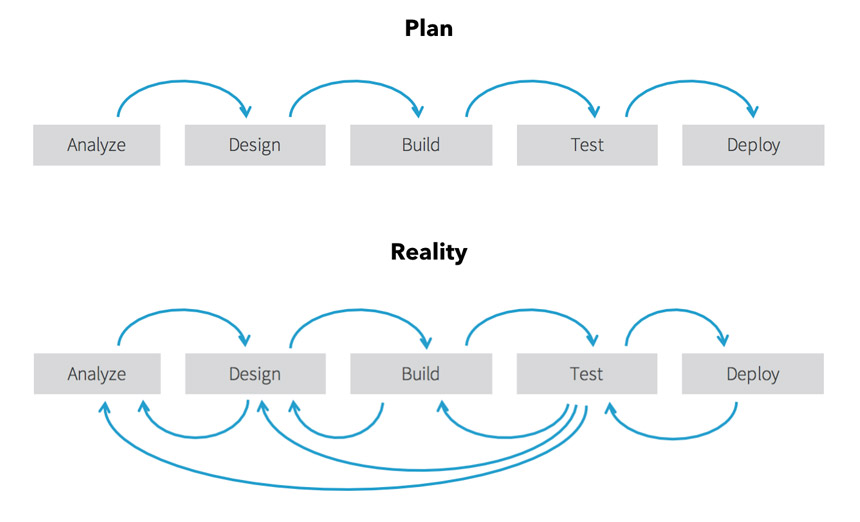
\includegraphics[width=\textwidth , keepaspectratio]{plan-vs-reality.jpg}
\centering
\caption{Rischi di pianificazione nell'attività di codifica.} 
\source{\href{https://www.devbridge.com/}{Devbridge.com}}
\label{fig:plan-vs-reality}
\end{figure}

\subsection{Vincoli metodologici}
%- monday meeting\\
%- interazione diretta con il cliente\\
%- scrum\\
%- Vincoli metodologici personali
Al mio arrivo in azienda, il progetto già presentava un'architettura e una metodologia di lavoro consolidate.
Data la mia poca esperienza con il \textit{framework} Scrum, in accordo unanime tra tutto il team, abbiamo deciso di mantenere la durata degli Sprint pari a due settimane lavorative, ma di inserire a metà di questo lasso di tempo una riunione che aveva la funzione di monitorare l'andamento dello sviluppo e di rilevarne eventuali criticità. I \textit{meeting} di \textit{Sprint Review} erano spesso presenziati anche dal comparto tecnico o dalle persone di riferimento delle aziende \textit{stakeholder}, così da avere un \textit{feedback} su quanto fatto finora pressoché istantaneo.
A questi inoltre, si aggiunge la politica aziendale del \textit{Monday Meeting}, ovvero una assemblea, effettuata ogni due Lunedì, nel corso del quale si aggiornano i colleghi sull'andamento dei progetti in corso.
Nonostante avessi carta bianca sulla modalità di sviluppo del codice, mi sono posto dei vincoli da rispettare, affinchè l'attività risultasse il più efficiente ed efficace possibile.\\
Innanzitutto, ho scelto di seguire un approccio di sviluppo differente da quello classico, ovvero il \textit{TDD}. Acronimo di \textit{Test Driven Development}, consiste nel rovesciare il normale metodo di programmazione, in cui prima si codifica e poi si effettuano i test, obbligando così lo sviluppatore a scrivere il codice in base ai test che sono stati realizzati in precedenza.
\begin{figure}[h]
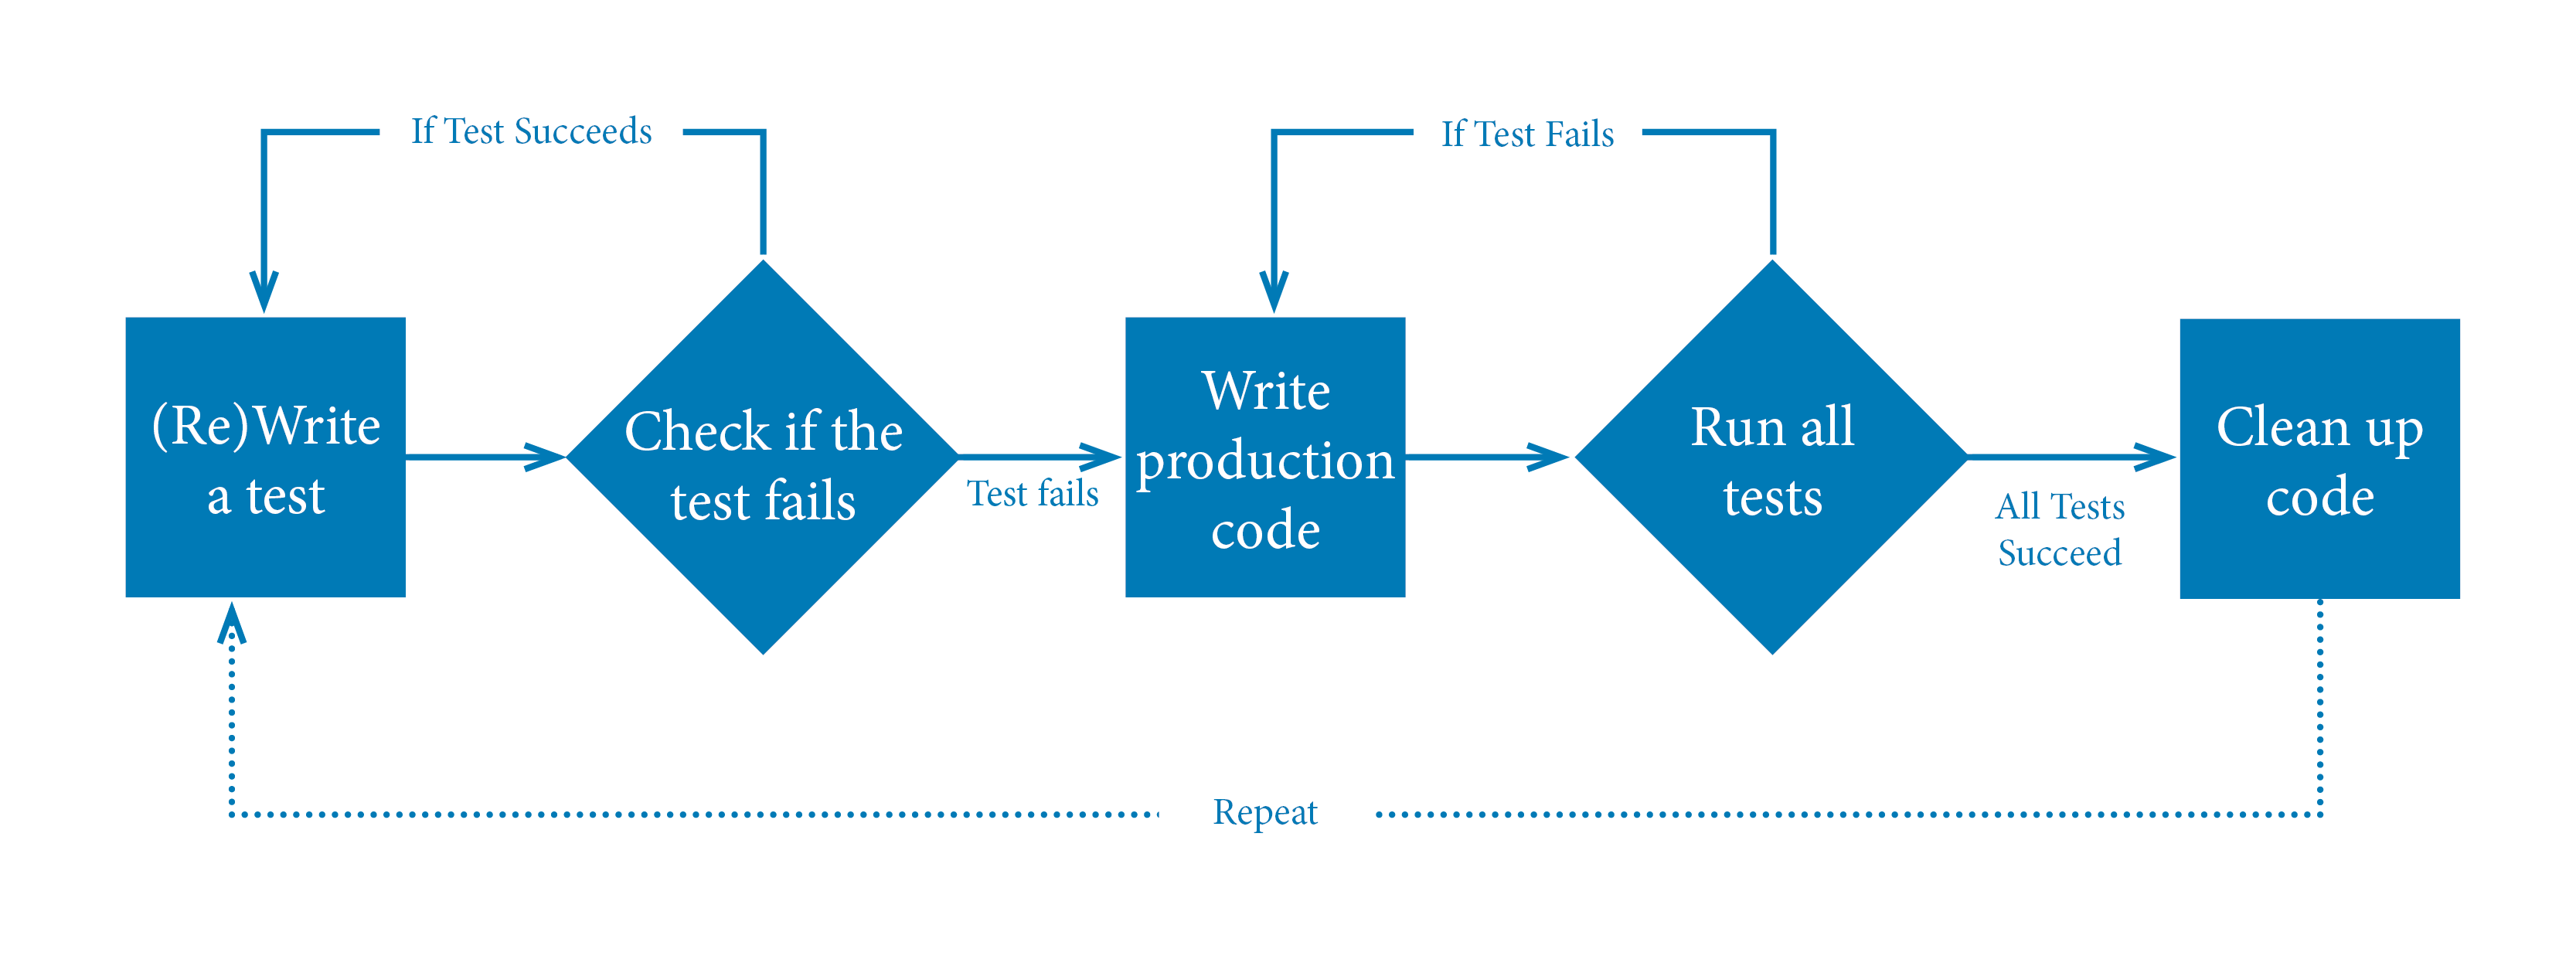
\includegraphics[width=\textwidth , keepaspectratio]{TestDrivenDevelopment.png}
\centering
\caption{Test Driven Development.} 
\source{\href{https://www.andplus.com/}{Andplus.com}}
\label{fig:tdd}
\end{figure}
In secondo luogo, ho configurato, tramite il \textit{framework} Jenkins, una \textit{pipeline} per la \textit{continuous integration} che eseguisse in maniera automatica i test precedentemente codificati.
Infine adottato il \textit{framework} \textbf{Swagger.io} per la documentazione delle chiamate \textit{API}.
%%%%%%%%%%%%%%%%%%%%%%%%%%%%%%%%%%%%%%%%%%%%%%%%%%%%%%%%%%%%%%%%%%%%%%%%%%%%%%%%%%%%%%%%%%%
\subsection{Vincoli tecnologici}
%stack tecnologico definito in avvio di progetto 

Per la realizzazione dei due progetti di stage, ho utilizzato due \textit{stack} tecnologici molto simili, ma per certi aspetti radicalmente differenti.\\
Il progetto \textbf{AWMS} si basa su tecnologie ampiamente utilizzate in azienda: 
\begin{itemize}
\item \textbf{PostgreSQL:} database relazionale, compatibile con il paradigma SQL, che consente all'utente di immagazinare dati anche in formato Json, rendendo di fatto il contenuto delle tabelle molto più dinamico;
\item \textbf{CakePHP:} \textit{framework} che consente lo sviluppo rapido di applicazioni web con architettura MVC. Grazie alla sua funzione di \textit{ORM}, permette di effettuare operazioni sulle tabelle trattando quest'ultime come oggetti derivanti dal paradigma \textit{OOP};
\item \textbf{Angular2+:} \textit{framework} per lo sviluppo di applicazioni web \textit{single-page}.
\end{itemize}
\textbf{DigitalSnapshots} invece si differenzia da AWMS in quanto sostituisce \textbf{MySQL} a \textit{PostgreSQL} e \textbf{AngularJS} ad \textit{Angular2+}.\\
Questa differenza di comparto tecnico è giustificata dal fatto che, mentre AWMS verrà seguito da \AD{} (nello specifico, da \textbf{I4.0Saas} dal 2020) per tutto il suo ciclo di vita, \textbf{DigitalSnapshots} avrà un destino differente: le fasi di progettazione e sviluppo sono a carico di \AD{}, mentre la fase di manutenzione del codice sarà eseguita dal reparto tecnico di Electrolux, committente del progetto.\\
Dai vincoli metodologici personali, deriva l'utilizzo dei \textit{framework} \textit{Jenkins}, per l'implementazione della \textit{continous integration}, e \textit{PHPUnit} e \textit{Jasmine} per l'esecuzione automatica dei test d'unità ed integrazione, rispettivamente per i linguaggi di programmazione PHP e Typescript.
\section{Aspettative personali}
%- come ho conosciuto AD\\
%- perchè AD?\\
%- aspettative sul lavorare in una startup, imparare il way of working\\
Durante l'ultimo anno del mio percorso accademico, ho avuto l'opportunità di partecipare a \textit{Stage-IT}, un evento organizzato da Assindustria Venetocentro in collaborazione con l'Università di Padova, con lo scopo di fornire un punto di contatto tra gli studenti e le aziende del settore informatico presenti nel territorio.
E\` proprio durante questo incontro che ho conosciuto \AD , e subito sono rimasto intrigato dalla sua dinamicità e propensione all'innovazione, nonché dai progetti ambiziosi e dai valori aziendali nei quali mi identifico.\\
\begin{figure}[h]

\includegraphics[width=\textwidth]{startup.jpg}
\centering
\caption{Le molte sfaccettature delle start-up.} 
\source{\href{http://orizzonti.tv/}{Orizzonti.tv}}
\label{fig:tdd}
\end{figure}
Le mie aspettative riguardo a questa attività di stage potevano essere riassunte in tre punti fondamentali:
\begin{itemize}
\item Innanzitutto, vedevo questo tirocinio come un banco di prova su cui testare le conoscenze acquisite durante il percorso universitario e la mia capacità di apprendimento di tecnologie a me perlopiù sconosciute;
\item In secondo luogo, ero smanioso di collaborare con aziende dal marchio rinomato, come Electrolux e Safilo.
\item Infine, ma non per questo meno importante, desideravo imparare il \textit{way of working} da persone con esperienza nel settore, perchè credo che conoscere gli strumenti e saperli utilizzare al meglio sia fondamentale per uno sviluppatore, specie se inesperto.
\end{itemize}
%%%%%%%%%%%%%%%%%%%%%%%%%%%%%%%%%%%%%%%%%%%%%%%%%%%%%%%%%%%%%%%%%%%%%%%%%%%%%%%%%%%%%%%%%%%